\newcommand{\swaggerlogo}{\vcenteredhbox{
\includegraphics[height=0.07\textheight]{./img/tag_swagger.png}}}
\newcommand{\ramllogo}{\vcenteredhbox{
\includegraphics[height=0.07\textheight]{./img/tag_raml.jpg}}}
\newcommand{\blueprintlogo}{\vcenteredhbox{
\includegraphics[height=0.07\textheight]{./img/tag_apiblueprint.png}}}

\section{Model-First approach}

\subsection{Overview}

\subsubsection{Steps of REST Service Creation}

\begin{frame}[allowframebreaks]
	\frametitle{Steps of REST Service Creation}
	
	Supposing we already defined some \emph{logic architecture} of the system or we `simply' need to wrap some pre-existing SW:
	\setbeamertemplate{enumerate items}[default]
	\begin{enumerate}
		\item Define the mean(s) for user/caller authentication
		\item Identify \emph{resources} and HTTP \emph{verbs} they support
		\item Assign some \emph{route} (URI) to each resource
		\begin{itemize}
			\item Routes can contain one or more \emph{query parameters}
		\end{itemize}
		
		\framebreak
		
		\item For each method supported by each route:
		\begin{enumerate}
			\item Choose one ore more needed authentication means
			\item Define supported request/response \emph{content-types}
			\begin{itemize}
				\item \texttt{application/json}, \texttt{application/xml}, \texttt{text/html}, \ldots			
			\end{itemize}
			\item Define \emph{where} to put \emph{request's arguments}
			\begin{itemize}
				\item Headers, Body, URI, Query	
			\end{itemize}
			\item Define request's arguments \emph{structures}
			\begin{itemize}
				\item \emph{JSON Schema}, \emph{DTD}, \emph{XML Schema}, \ldots
			\end{itemize}
			\item Define \emph{status codes} allowed as \emph{responses} and, for each one:
				\begin{itemize}
					\item \emph{Body}'s structure
					\item \emph{Headers}' structure
				\end{itemize}
		\end{enumerate}
	\end{enumerate}
	
	\framebreak
	
	\begin{exampleblock}{Example: Pet Store - API Routes}
		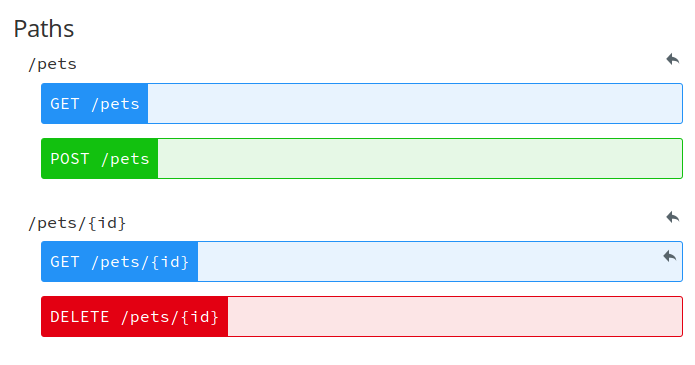
\includegraphics[width=\textwidth]{./img/api_example_paths_alpha.png}
	\end{exampleblock}
	
	\framebreak
		
	\begin{exampleblock}{Example: Pet Store - Route Detail}
		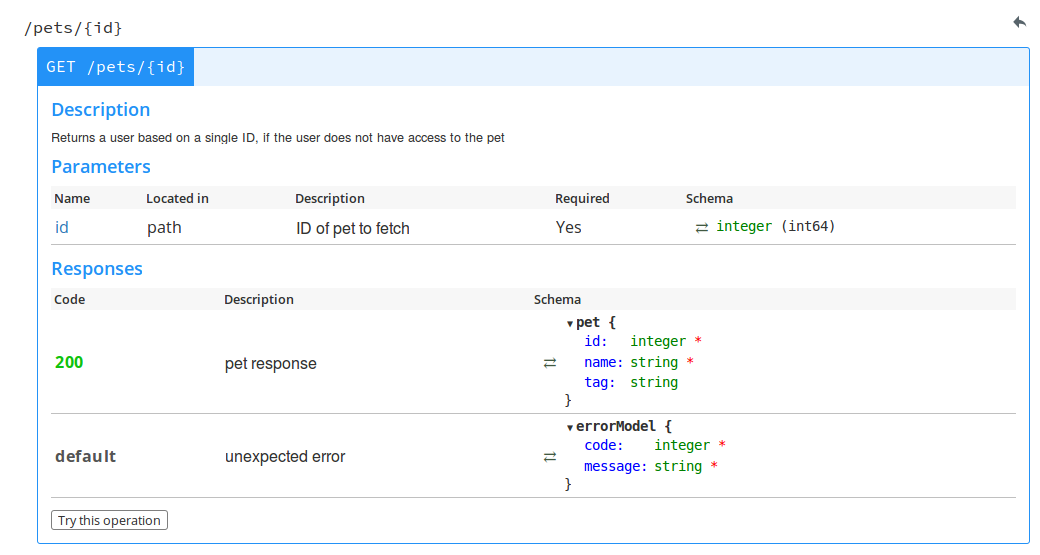
\includegraphics[width=\textwidth]{./img/api_example_route_alpha.png}
	\end{exampleblock}
	
	\framebreak
			
	\begin{exampleblock}{Example: Pet Store - JSON Schemas (Tiping)}
		\begin{tabularx}{\textwidth}{X||X}
			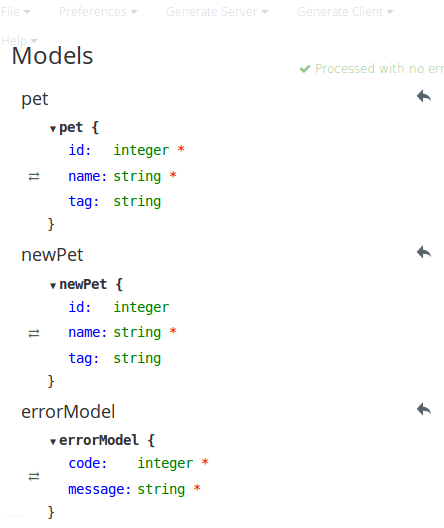
\includegraphics[width=0.48\textwidth]{./img/api_example_schemas1_alpha.png} &
			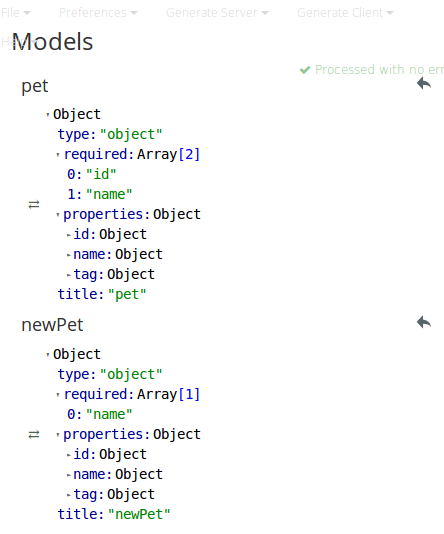
\includegraphics[width=0.48\textwidth]{./img/api_example_schemas2_alpha.png}
		\end{tabularx}
	\end{exampleblock}
	
\end{frame}

\subsubsection{Model-first tools}

\begin{frame}[allowframebreaks]
	\frametitle{Model-first tools}
	
	What if we had some formal way to model APIs?
	
	\begin{exampleblock}{Swagger}
		 \swaggerlogo\ \url{http://swagger.io}
	\end{exampleblock}
	
	\begin{exampleblock}{RAML - \textbf{R}ESTful \textbf{A}PI \textbf{M}odelling \textbf{L}anguage}	
		\ramllogo\ \url{http://www.raml.org}
	\end{exampleblock}
	
	\begin{exampleblock}{Api Blueprint}
	 	\blueprintlogo\ \url{https://apiblueprint.org/}
	\end{exampleblock}
	
	\framebreak
	
	\begin{block}{Desired facilities}
		\begin{description}
			\item[Specification Language :] allows formal (machine-readable) and intellegible (human-readable) API specification
			\item[API Console :] some sort of GUI allowing for APIs navigation (usually Web-based)
			\item[Mock server :] proxy server whose code is generated using some formal specification; it validates clients' requests and forwards them to some other server responsible for business-logic implementation
			\item[Server stub :] code stubs generated using some formal specification for some particular platform (e.g. \texttt{express-js}); clients' requests validation is performed by the generated code, programmers only have to implement business-logic
			\item[] \ldots
		\end{description}
	\end{block}
\end{frame}

\subsubsection{Users Example}

\begin{frame}[allowframebreaks]
	\frametitle{Users Example}
	
	In order to compare the three technologies the `Users' minimal API has been modelled using each language.
	
	\begin{block}{Resources and methods informal description pt. 1}
		\begin{description}
			\item[\texttt{/users} :] The set of registered users
			\begin{description}
				\item[\texttt{GET} :] Retrieves public informations for a number of users
				\item[\texttt{POST} :] Creates one user
			\end{description}
			\item[\texttt{/users/\{username\}} :] The specific user whose username is specified within the path
			\begin{description}
				\item[\texttt{GET} :] Retrieves informations about the specific user \emph{[requires authentication]}
			\end{description}
		\end{description}
	\end{block}
	
	\framebreak
	
	\begin{block}{Resources and methods informal description pt. 2}
		\begin{description}
			\item[\texttt{/users/\{username\}/token} :] The authentication token for a specific user
			\begin{description}
				\item[\texttt{POST} :] Creates and returns one signed JWT if the provided username and password (within request's body) are correct
			\end{description}
		\end{description}
		\vspace{5mm}
		\begin{itemize}
			\item Authentication: signed JWT within the \texttt{Authorization} header identifies the users 
			\item It's an example! Let's suppose HTTP it's secure.
		\end{itemize}
	\end{block}
	
	
	
\end{frame}